\section{Varying Lengths and Mass Flowrate}
%
When the design team varied the lengths of the heat exchanger for one tube, the results were interesting. From the results, seen in the figure below, as the length of the tube got longer the hot outlet temperature decreased. However for the cold water leaving the system, the temperature coming out had the opposite effect. As the length of the tube increased the temperature increased and as the mass flow rate ratio increased the temperatures all converged to relatively the same range of temperatures, thus the mass flow rate has little impact after a mass flow ratio of 7. 
%
\begin{figure}[H]
    \centering
    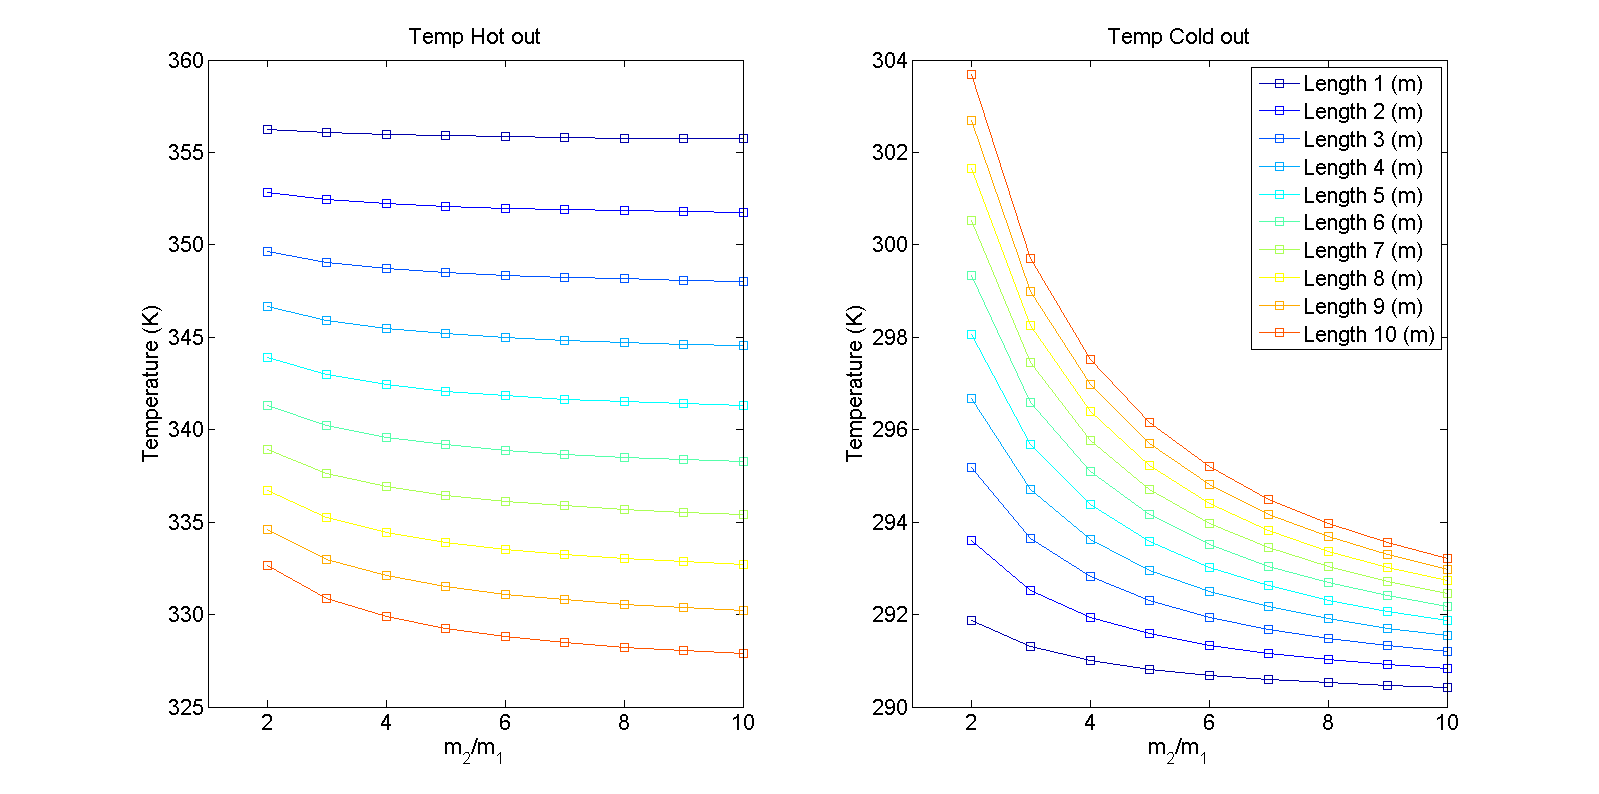
\includegraphics[height=3in]{pictures/part_3_single_temp_len_mass.png}
\end{figure}
%
\noindent
To see how effectiveness changes in a parallel system, the number of tubes of varying length in the system will be compared to the overall effectiveness. As seen in the figure below, as the length of the tube increased from one to ten meters, so did the effectiveness. Like before, the effectiveness drops significantly due to the fact that the Reynolds number changes due to the transition to laminar flow in the outer tube. This shows that for an efficient design a heat exchanger with approximately 22 tubes and a length of 10 meters will result in the most effective heat exchanger. This configuration is optimal because each fluid stream is still in turbulance and has the lowest mass flowrates.
%
\begin{figure}[H]
    \centering
    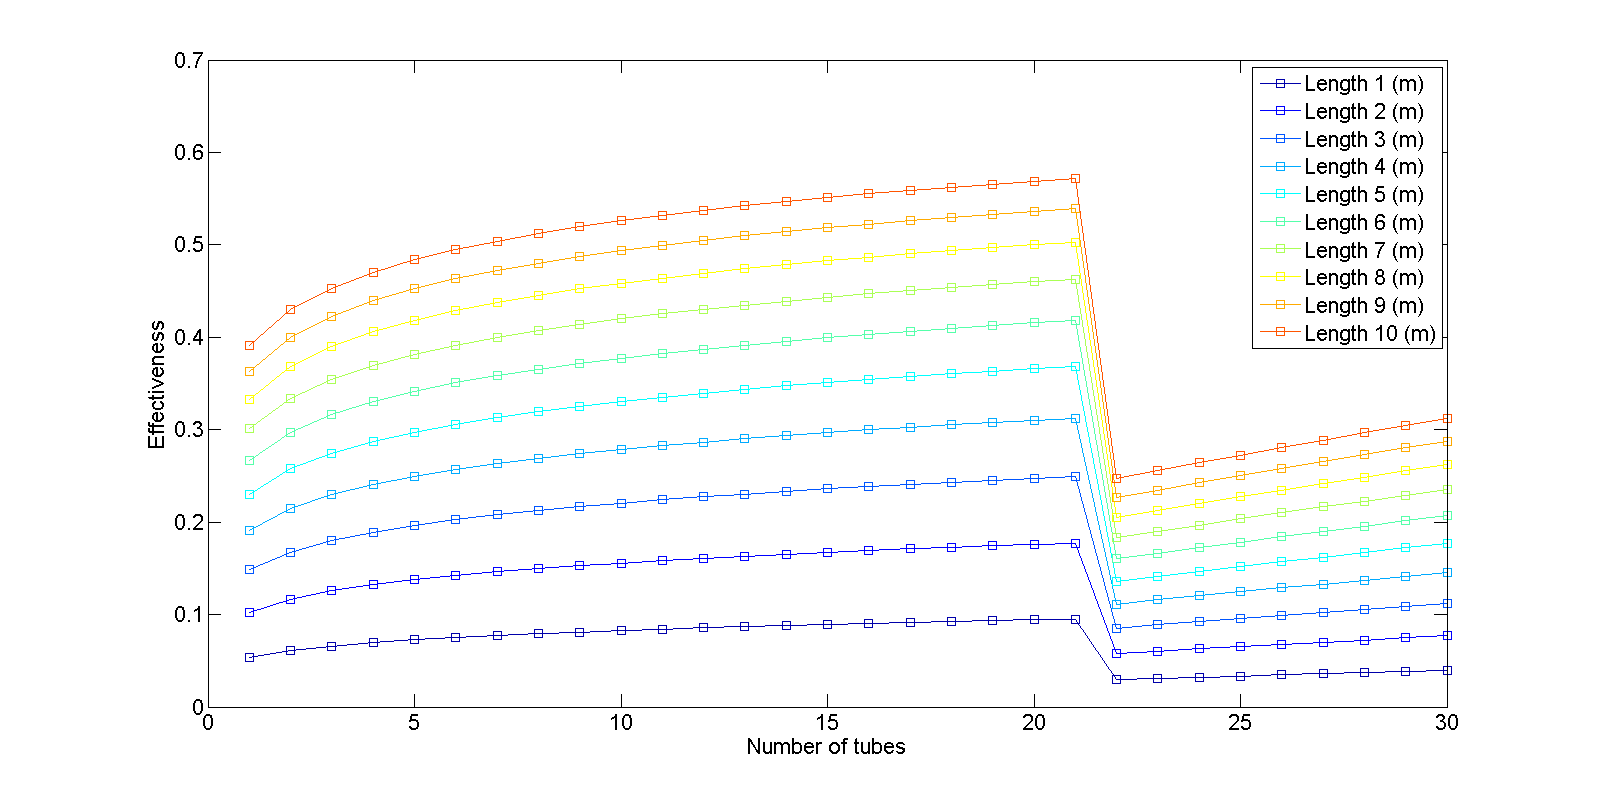
\includegraphics[height=3in]{pictures/part_3_eff_tubes_length.png}
\end{figure}
%




